\section{L'équipe de Data Publica}
    \subsection{L'équipe technique}
    \label{annexe:teamd_data_publica}
        L'équipe technique de Data Publica est visible en figure \ref{fig:teamd_data_publica}.
        \begin{figure}[h!]
            \centering
            \begin{subfigure}[b]{0.2\textwidth}
                
\includegraphics[width=\textwidth]{images/christian-serieux.png}
                \caption{Christian F.}
                \label{fig:christian}
            \end{subfigure}
            \begin{subfigure}[b]{0.2\textwidth}
                
\includegraphics[width=\textwidth]{images/thomas2-Copier-Copier.jpg}
                \caption{Thomas D.}
            \end{subfigure}
            \begin{subfigure}[b]{0.2\textwidth}
                
\includegraphics[width=\textwidth]{images/guillaume-serieux.png}
                \caption{Guillaume L.}
            \end{subfigure}
            \begin{subfigure}[b]{0.2\textwidth}
                
\includegraphics[width=\textwidth]{images/samuel-serieux.png}
                \caption{Samuel C.}
            \end{subfigure}
            \begin{subfigure}[b]{0.2\textwidth}
                
\includegraphics[width=\textwidth]{images/loic-serieux.png}
                \caption{Loïc P.}
            \end{subfigure}
            \begin{subfigure}[b]{0.2\textwidth}
                
\includegraphics[width=\textwidth]{images/clement-c-serieux.png}
                \caption{Clément C.}
            \end{subfigure}
            \begin{subfigure}[b]{0.2\textwidth}
                
\includegraphics[width=\textwidth]{images/clement-d-serieux.png}
                \caption{Clément D.}
            \end{subfigure}
            %\begin{subfigure}[b]{0.2\textwidth}
            %    
\includegraphics[width=\textwidth]{images/jacques.jpg}
            %            \caption{Jacques B.}
            %\end{subfigure}
            \begin{subfigure}[b]{0.2\textwidth}
                
\includegraphics[width=\textwidth]{images/vincent.jpg}
                \caption{Vincent Y.}
            \end{subfigure}
            \caption{L'équipe technique de Data Publica}
            \label{fig:teamd_data_publica}
        \end{figure}

\newpage

    \subsection{L'équipe commerciale}
    \label{annexe:teamc_data_publica}
        L'équipe commerciale de Data Publica est visible en figure \ref{fig:teamc_data_publica}.
        \begin{figure}[h!]
            \centering
            \begin{subfigure}[b]{0.2\textwidth}
                
\includegraphics[width=\textwidth]{images/francois-serieux.png}
                \caption{François B.}
                \label{fig:francois}
            \end{subfigure}
            \begin{subfigure}[b]{0.2\textwidth}
                
\includegraphics[width=\textwidth]{images/emmanuel-serieux.png}
                \caption{Emmanuel J.}
            \end{subfigure}
            \begin{subfigure}[b]{0.2\textwidth}
                
\includegraphics[width=\textwidth]{images/philippe-1-serieux.png}
                \caption{Philippe S.}
            \end{subfigure}
            \begin{subfigure}[b]{0.2\textwidth}
                
\includegraphics[width=\textwidth]{images/Justine-serieuse-crop.jpg}
                \caption{Justine P.}
            \end{subfigure}
            \caption{L'équipe commerciale de Data Publica}
            \label{fig:teamc_data_publica}
        \end{figure}

\section{Dataviz}
\label{annexe:firmo}
    Un exemple de dataviz est présenté en figure \ref{fig:firmo}.
    \begin{figure}[h!]
        \centering
        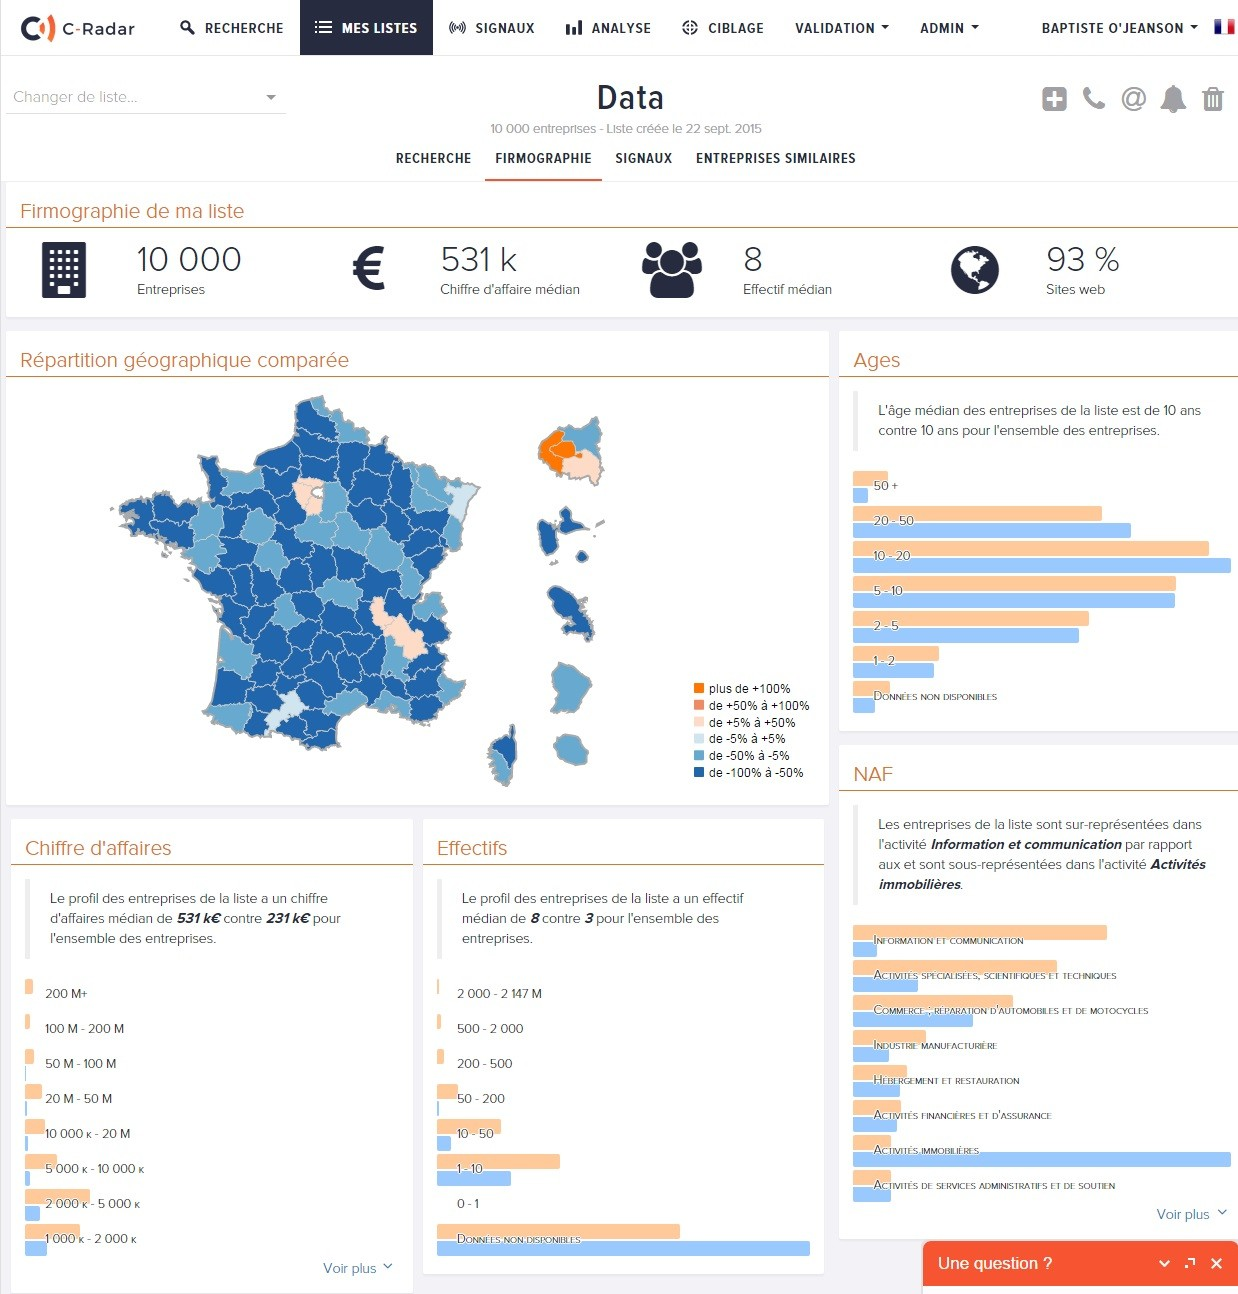
\includegraphics[width=\textwidth]{images/firmo.jpg}
        \caption{Exemple de Dataviz : Firmographie dans C-Radar}
        \label{fig:firmo}
    \end{figure}

\section{La validation croisée et les hyper-paramètres}
\label{annexe:cv}

\section{Les métriques de mesure de la qualité d'une classification}
    \subsection{Terminologies}
        Pour une classe donnée, voici la signification de ces terminologies :
        \begin{itemize}
            \item $\highlight[green]{TP}$ : True positive, bonne assignation à la classe ;
            \item $\highlight[green]{TN}$ : True negative, bon rejet de la classe ;
            \item $\highlight[red]{FP}$ : False positive, mauvaise assignation à la classe ;
            \item $\highlight[red]{FN}$ : False negative, mauvais rejet de la classe.
        \end{itemize}

    \subsection{La précision}
    \label{annexe:precision}
        Pour une classe donnée, la précision est le nombre de documents correctement assignés à cette classe rapporté au nombre de documents total assignés à cette classe par le classifieur.\\
        $Précision\ =\ \frac{TP}{TP+FP}$


    \subsection{Le rappel}
    \label{annexe:rappel}
        Pour une classe donnée, le rappel est défini par le nombre de documents correctement assignés à cette classe au regard du nombre total de documents appartenant réellement à cette classe.\\
        Le rappel mesure le fait que le classifieur ait trouvé tous les documents d'une classe.\\
        $Rappel\ =\ \frac{TP}{TP+FN}$

\section{Le QA ou Quality Assessment}
\label{annexe:qa}
    L'objectif du QA est de demander la contribution d'un maximum de personnes sur une tâche de validation manuelle pénible.\\

\section{Modèle de classifieur}
    Les points d'explication qui suivent, sont en partie tirés de Wikipédia\autocite{wiki_discri_gene}.
    \subsection{Le modèle génératif}
    \label{annexe:generatif}
        Le modèle génératif consiste à modéliser les probabilités conditionnelles soit $P(donnée | classe)$. Voici quelques exemples d'algorithmes de ce type :
        \begin{itemize}
            \item Classifieur naïf bayésien implique une distribution de probabilité conditionnelle de type binomiale (ou multinomiale) ;
            \item Analyse discriminante linéaire (LDA). Elle implique l'existence d'un modèle discriminant basé sur une distribution de probabilité de type Gaussienne.
        \end{itemize}
        Le modèle génératif maximise la vraisemblance de la probabilité jointe $P(classe, donnée)$.

    \subsection{Le modèle discriminant}
    \label{annexe:discriminatif}
        Le modèle discriminant cherche à maximiser la qualité de la classification. Une fonction de coût va réaliser l'adaptation du modèle de classification (en minimisant les erreurs). Voici quelques exemples d'algorithmes de ce type :
        \begin{itemize}
            \item Régression logistique, maximisation de la vraisemblance en considérant que les données suivent un modèle binomial ;
            \item Support Vectort Machine (SVM), maximisation de la marge entre l'hyperplan séparant les données.
        \end{itemize}
        Le modèle discriminant maximise la vraisemblance de la probabilité conditionnelle $P(classe | donnée)$.

\section{Les transducteurs}
\label{annexe:transducteurs}
    Définition tirée de Wikipédia\autocite{wiki_trans}.\\

    En informatique théorique, en linguistique, et en particulier en théorie des automates, un transducteur fini (appelé aussi transducteur à états finis par une traduction maladroite de l'anglais finite state transducer) est un automate fini avec sorties. C'est une extension des automates finis. Ils opèrent en effet sur les mots sur un alphabet d'entrée et, au lieu de simplement accepter ou refuser le mot, ils le transforment, de manière parfois non déterministe, en un ou plusieurs mots sur un alphabet de sortie. Ceci permet des transformations de langages, et aussi des utilisations variées telles que notamment l'analyse syntaxique des langages de programmation, et l'analyse morphologique ou l'analyse phonologique en linguistique.\\

    D'autres explications détaillées sont disponibles \href{http://sixty-north.com/blog/deriving-transducers-from-first-pr}{ici}.